 \documentclass{article} %A4
\usepackage[a4paper,left=1.9cm, right=2.1cm,top = 1.2cm,bottom=2.3cm]{geometry}
\usepackage[utf8]{inputenc}%Umlaute
\usepackage[ngerman]{babel} %Texttrennung
\usepackage{graphicx}	%Grafiken
\usepackage{amssymb}
\usepackage{amsmath}
\usepackage{url}
\usepackage{listings}
 \usepackage{color}
\usepackage{hyperref}
\usepackage{framed}
\usepackage{algpseudocode}
\usepackage{tikz}

\usepackage[labelformat=empty]{caption}
\title{Zusammenfassung - NASS}
\author{
	SK
}

\begin{document}
\maketitle
\begin{framed}
	Korrektheit und Vollständigkeit der Informationen wird nicht gewährleistet.
\end{framed}
\setcounter{tocdepth}{1}
\tableofcontents

\section{Introduction}
\subsection{Taxonomie der Angreifer}
\begin{itemize}
	\item einzelner Angreifer
    
    \begin{itemize}
        \item sozialer Hintergrund
        \item öffentliche Aufmerksamkeit als Antrieb
        \item evtl pol. Statements
        \item geht gewöhnlich niedrige Risiken ein
    \end{itemize}
    \item organisierte Kriminalität
    
    \begin{itemize}
        \item Geld als Antrieb
        \item mittlere Risiken
    \end{itemize}
    \item Terroristen
    
    \begin{itemize}
        \item politische oder gesellschaftliche Motivation
        \item hohe Risiken
        \item Zerstörung/Verwirrung als Ziel
    \end{itemize}
    
    \item Konkurrenten
    
    
    \begin{itemize}
        \item möglichst niedriges Risiko der Aufdeckung(abhängig vom wert der Information)
        \item Informationsdiebstahl oder Zerstörung als Ziel
    \end{itemize}
    
    \item Regierungsorganisationen
    
    
    \begin{itemize}
        \item Industriespionage zum Wohl einheimischer Firmen
        \item Militärspionage udn hybride Kriegsführung
    \end{itemize}
\end{itemize}

\subsection{Angriffe gegen einen Computer}
Informationsdiebstahl führt zu:
\begin{itemize}
	\item Wettbewerbsvorteilen
    \item Verwirrung
    \item Erpressung
    
\end{itemize}
Zerstörung führt zu:
\begin{itemize}
	\item Spaß und Selbstverherrlichung
    \item Politischen Stellungnahmen
\end{itemize}
Sammlung von Informationen
\begin{itemize}
	\item Infos werden zu Angreifer gesendet
    \item an Netzwerk angeschlossene Rechner mit höherem Risiko
    \item Zugriff für Angreifer durch:
    
    \begin{itemize}
        \item Social engineering
        \item Viren/Trojaner/Würmer
        \item Physischer Diebstahl von Datenträgern
        \item Sniffing
    \end{itemize}
    
\end{itemize}
Zerstörung von Infos
\begin{itemize}
	\item Infos gehen verloren
    \item physische Angriffe/Feuer/Naturkatastrophen
    \item Beabsichtigte Löschungen durch 
    
    \begin{itemize}
        \item Social Engineering
        \item Viren/Trojaner/Würmer
    \end{itemize}
\end{itemize}
Viren
\begin{itemize}
	\item Infektion von Dateien 
    \item Infektion von System und Boot record
    \item Zerstörung, Verwirrung und öffentliche Aufmerksamkeit als Ziel
\end{itemize}
Würmer
\begin{itemize}
	\item Mailing Worms - Verbreitung durch E-Mails
    \item Viren/Trojaner evtl als "`Nutzlast"'
    \item Network worms - Verbreitung durch Ausnutzung von Softwaremängeln(bspw Bufferoverflows)
    \item Ablauf:
    
    \begin{itemize}
        \item Zielauswahl
        \item ausnutzen(exploit)
        \item Infektion
        \item Verbreitung
    \end{itemize}
\end{itemize}
Backdoors und Trojaner
\begin{itemize}
	\item Schadsoftware wird in nützlicher Software versteckt
    \item mögliche Funktionen:
    
    \begin{itemize}
        \item mitschneiden von Daten(logging)
        \item Zerstörung
        \item Installation weiterer Software(DoS Clients, root kits etc)
        \item bedingter Start von Prozessen (time bombs)
    \end{itemize}
\end{itemize}
Identitäts Spoofing
\begin{itemize}
	\item Angreifer übernimmt die Identität von jemand anderem 
    \item Angreifer und Ziel müssne normalerweise ein Netzsegment teilen
    \item Angreifer liefert evtl falsche Infos über Routen oder Namen
    \item Grundsätzlich sind alle Antworten eines Protokolls potentielle Spoofingsubjekte(subject of spoofing?)
\end{itemize}
DoS
\begin{itemize}
	\item Angreifer möchte einen Dienst der von einem Rechner oder Gerät angeboten wird überladen
    \item Angriffe gegen Konkurrenten, als pol/gesellschaftliche Aussage oder um andere Aktivitäten zu verbergen
    \item bösartige Anfragen sind nicht von normalen Anfragen zu unterscheiden
    \item BSP: HTTP, DNS DoS, SYN Flooding
\end{itemize}
Bot Network
\begin{itemize}
	\item Fernsteuerung mehrerer Rechner um bösartige Aktionen auszuführen
    \item bsp: DDoS, aufwändige Entschlüsselungen berechnen
\end{itemize}
Password/Schlüssel Attacken
\begin{itemize}
	\item Brute Force
    \item Raten/ Wörterbuchangriffe
    \item Mängel in der Implementation(z.B. Password als Klartext gespeichert)
\end{itemize}
Port/Network Scanning

\begin{itemize}
	\item während der Aufklärungsphase um Sicherheitslücken und geeignete Ziele zu finden
    \item Angreifer möchte Informationen über das System erlangen
    \item Sniffing/Mapping/Port Scans
\end{itemize}
Session Highjacking
\begin{itemize}
	\item Angreifer bricht in einen bestehender Session ein ohne sich einloggen zu müssen.
\end{itemize}

ZSF: viele unterschiedliche Angriffsmöglichkeiten $\Rightarrow$ unüberschaubare Anzahl an verschiedenen Attacken
Angreifer unterscheiden sich in Motivation und Möglichkeiten.


\section{Einführung und Rekapitulation}
\subsection{Sicherheitskomponenten}
\begin{itemize}
	\item Firewalls
    \item Intrusion Detection/Prevention Systems
    \item Proxies
    \item interne oder private Netzwerke / Netzwerkzonen / Entmilitarisierte Zonen
    \item VPNs
\end{itemize}
\subsection{Firewalls}
entscheidet ob Verkehr ins Netzwerk gelangen darf oder nicht
Typen: 
\begin{itemize}
	\item Paketfilter
    \item Zustandsbehaftete Firewall
    \item Proxyfirewall
\end{itemize}
\subsection{Intrusion Detection Systems}
Identifizierung von Attacken / verdächtigem Verkehr \\
Hilfe beim Einrichten/ konfigurieren von Firewalls \\
Normalerweise transparent für Nutzer und Angreifer.\\
hauptsächlich 2 Arten:
\begin{itemize}
	\item Mustererkennung
    \item Anomalieerkennung
\end{itemize}
\subsection{Proxies}
strickte Trennung von internen und externen Netz\\
Üblicherweise auf Application Layer. Verhindert dass bestimmte Informationen(Viren, Pornos, illegale Infos) in das interne Netz gesandt werden.\\
Verhindert, dass bestimmte Informationen nach außen gesendet werden.\\
Kombinationen mit anderen Systemen(Virenfilter/ Spamfilter / IDS...)\\
\subsection{VPN}
VPNs erschaffen einen gemeinsamen Addressraum.\\
VPNs schützen die Kommunikation über ungesicherte Netzwerke als würde sie in einem Netzwerk stattfinden.\\
Gegenseitige Authentifizierung der Kommunikationspartner.\\
VPNs bieten signifikante Einsparungen über dedizierte Verbindungen.
\subsection{Zonen - DMZ}
kleine Netzwerke, welche öffentlich erreichbare Dienste beeinhalten (z.B. HTTP)\\
DMZ oft durch Firewalls etc geschützt.\\
DMZ befinden sich außerhalb des internen Netzes.\\
sind unsicherer als das interne Netz.\\
Abgeschirmte Teilnetze sind isolierte Netze innerhalb des internen Netzes
\subsection{internes Netz}
eingeschränkter Zugriff auf das externe Netz nur über gut bekannte Ports\\
Internes Angriffsrisiko hängt ab von:
\begin{itemize}
	\item Anzahl der Nutzer
    \item Vertrauen in die Nutzer
    \item Zugriffswege der Nutzer(Notebooks?)
    \item Fähigkeiten der Nutzer
\end{itemize}
Hosts müssen trotzdem noch mit firewalls etc geschützt werden
\subsection{Basis Kryptografie}
Kerkhoff's Prinzip: Sicherheit hängt nur von Schlüssel ab und nicht von der Kenntnis der kryptografischen Funktion.\\
\subsubsection{symmetrische Verschlüsselung}
Beide Teilnehmer benutzen zum ver- und entschlüsseln denselben Schlüssel.\\
Stromchiffren: Klartext wird Zeichen für Zeichen ver- und entschlüsselt.\\
Blockchiffren: arbeitet mit festen Blockgrößen und entschlüsselt mehrere Zeichen in einem Schritt.\\
\paragraph{One-Time Pads}
Stromchiffre deren Schlüsselstrom ein Strom aus echten Zufallsbits ist\\
Uneingeschränkt sicher(einziges bisher "`bewiesen"' sicheres Verfahren).\\
Schlüssel muss zu verschlüsseln mindestens so lang sein wie der Klartext.\\
Jeder Schlüssel darf nur einmal verwendet werden.\\
Nachteil: viel Speicherbedarf für Schlüssel.\\
\subsubsection{asymmetrische Verschlüsselung}
Sender und Empfänger nutzen jeweils unterschiedliche Schlüssel.\\
Es ist schwierig den Entschlüsselungsschlüssel(k') aus dem Verschlüsselungsschlüsselungsschlüssel(k) zu berechnen\\
k kann öffentlich gemacht werden (public-key-Verschlüsselung).\\
Nachteil: Verteilung der Schlüssel\\
\subsubsection{hybride Verschlüsselung}
Kombination aus symmetrischer udn asymmetrischer Verschlüsselung.\\
symmetrischer Session Key mit dem die Daten symmetrisch verschlüsselt werden.\\
Session Key wird asymmetrisch mit public Key des Empfängers verschlüsselt.\\
löst Verteilungsproblem der asymmetrischen und behält Geschwidigkeit der symmetrischen Verschlüsselung\\
\subsubsection{kryptografische Hashfunktion}
Anforderungen:
\begin{itemize}
	\item einseitig: wenn Hashwert y gegeben ist, ist es rechnerisch unmöglich eine Nachricht x zu finden, sodass h(x) = y
    \item schwacher Kollisionswiderstand: bei gegebener Nachricht ist es rechnerisch unmöglich eine andere Nachricht mit gleichem Hashwert zu finden
    \item starker Kollisionwiderstand: Es is rechnerisch unmöglich zwei Nachrichten mit gleichem Hashwert zu finden.
\end{itemize}
\paragraph{Hash und Signaturen}
Von Nachricht wird Hash gebildet. Dieser wird verschlüsselt und als Signatur an die Nachricht gehängt.\\
Empfänger entschlüsselt Signatur mit public key des Senders und vergleicht mit dem hash der Nachricht. Wenn gleich dann ist alles gut, wenn nicht dann wurde was verändert.\\
\subsubsection{Diffie-Hellman Schlüsselaustausch}
\begin{figure}[h]
	\centering
		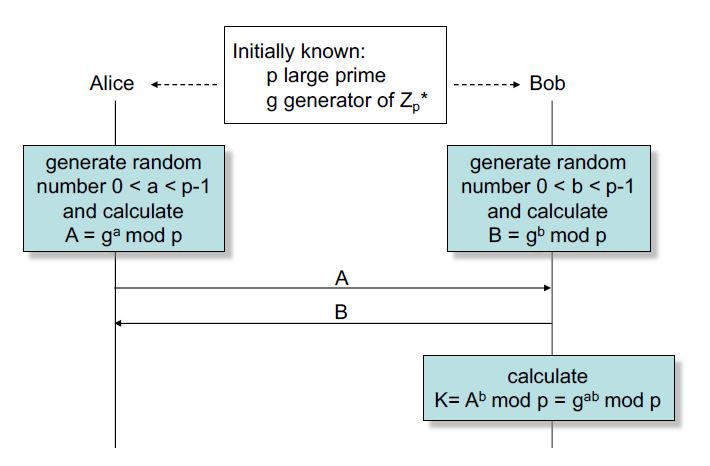
\includegraphics[width=8cm]{img/diffiehellman.JPG}
	\label{fig:diffiehellman}
\end{figure}


\subsubsection{Zertifikate}
Zertifikat ist eine Datenstruktur welche folgendes enthält:
\begin{itemize}
	\item Öffentlichen Schlüssel
    \item Namen des Eigentümers des öff Schlüssels
    \item Namen des Ausstellers
    \item Ausstellungsdatum
    \item Ablaufdatum
    \item Möglicherweise andere Daten
    \item Signatur des Ausstellers
\end{itemize}
\subsubsection{Certification Authorities (CA)}
stellen Zertifikate aus.\\
sind normalerweise vertrauenswürdige Dritte.\\
Zertifikate werden über online Datenbanken verteilt(Certificate Directories) denen vertraut werden muss.


\section{Paketfilter}
 \subsection{Funktionsweise von Paketfiltern}
Netzwerkpakete werden akzeptiert oder zurückgewiesen anhand von Parametern wie:
\begin{itemize}
	\item Quelladresse/Ports
    \item Zieladresse/Ports
    \item Flags
\end{itemize}
\subsection{Paketfilterregeln}
Regeln können bzgl Flags, Adressen und Ports angewandt werden.\\
Paketfilter können auch bezüglich des Inhaltes von Paketen angewandt werden.\\
Zulassende Regeln:
\begin{itemize}
	\item explizites Erlauben von Zugriff
    \item sämtlicher anderer Verkehr wird verhindert
\end{itemize}
Verhindernde/ablehnende Regeln:
\begin{itemize}
	\item bestimmter Verkehr wird explizit abgelehnt.
    \item sämtlicher anderer Verkehr wird für gewöhnlich zugelassen.
\end{itemize}
Wichtig:
\begin{itemize}
	\item Reihenfolge der Regeln ist wichtig.(erst alles verhindern und dann einige zulassen ist was anderes als erst einige zulassen und dann alles zu verhindern!)
    \item große Anzahl an Regeln kann verwirrend sein.
    \item "`alles verbieten und solange es nicht explizit benötigt wird"' kann gute Herangehensweise sein.
\end{itemize}
\subsubsection{Ingress-Filter}
Filtern ankommende Pakete\\
blockieren Zugriff von verdächtigen Quelladdressen.\\
 \subsubsection{Egress-Filter}
Filtern ausgehenden Verkehr.\\
Nur Pakete mit Quelladdresse im Netzwerk dürfen das Netzwerk verlassen so lange keine andere Regel greift.\\
Quellen von abgewiesenen Paketen sind gute Kandidaten für Überprüfung.\\
\subsubsection{Protokollfilter}
Dienste haben haben festgelegte Protokolle\\
Daumenregel: nur Verkehr zu Diensten zulassen die wirklich benötigt werden.\\
\subsubsection{Probleme}
Zugriff für bestimmte Netze zulassen\\
Gefahr des Spoofings: Angreifer nutzt evtl falsche Quelladressen\\
Source Routing: 
\begin{itemize}
	\item Pakete enthalten evtl Infos über die Route zurück zum Urheber
    \item Überschreiben die Routingtabelle des Routers
\end{itemize}
Gefahr das Filterregeln umgangen werden\\
Fragmentierung:
\begin{itemize}
	\item Paketfilter untersuchen Headerinfos
    \item Paket wird so aufgeteilt dass der Header geteilt wird und Adresse und Ports nicht gefiltert werden können.
\end{itemize}
Löcher:
\begin{itemize}
	\item Dienste müssen erreichbar bleiben für externe Netzwerke
    \item entsprechende Ports müssen geöffnet werden.
\end{itemize}
\subsection{dynamische Paketfilter}
Filterregeln werden on the fly so erstellt wie sie benötigt werden und nach schließen der Verbindung wieder gelöscht.\\
Filter beobachten ausgehenden Verkehr und erstellen zurückwirkende Regeln.(Ausgehender Verkehr zu einer Adresse bewirkt Regel dass eingehender Verkehr von dieser Adresse erlaubt wird.)\\
Probleme: 
\begin{itemize}
	\item Regeln sind angreifbar z.B. durch senden falscher reset Pakete
    \item ausgehender Verkehr wird nicht gefiltert. Gefahr von Trojanern/Viren.
\end{itemize}


\section{Zustandsbehaftete Firewalls}
\subsection{Funktionsweise}
Kennen den Zustand von Verbindungen und wissen welche Pakete in welchem Zustand erwartet werden.\\
Es können Regeln angewandt werden die nur in bestimmten Zuständen wirksam sind.\\
Untersuchen hauptsächlich  OSI 4 (transport layer), aber auch höhere Schichten.\\
\subsection{Probleme}
Hohe Leistung benötigt teilweise geclusterte Hardware. Zustandsbehaftete Firewalls lassen sich nicht einfach clustern.\\
Zustandslose Protokolle (UDP, ICMP, DNS, HTTP)\\
\subsubsection{Zustandslose Protokolle}
Zustandslose Protokolle definieren trotdem welche Pakete erwartet werden.\\
Timeouts werden genutzt um Pseudo-Verbindungen zu erzeugen.\\
\subsection{Multi-Layer Inspection}
Die meisten Protokolle basieren auf Protokollen aus niedrigeren Layern. BSP: HTTP nutzt TCP Verbindungen.\\
Zustandsbehaftete Firewalls können beide Layer beobachten.


\section{Proxy Firewalls}
%050_Proxy_Firewalls.pdf
Proxies verhalten sich für den inneren Client wie der äußere Server und andersherum. Client und Server werden niemals direkt miteinander agieren. Der Proxy ist außerdem intransparent. Auf dem Proxy selbst können ein paar Programme laufen, die sicher sind und denen vertraut werden kann.\\
Proxies können die interne Struktur eines Netzwerkes nach außen hin verstecken und gegen Protokoll-Angriffe schützen. Forward Proxies sind ein Mittel, um ausgehenden Traffic zu kontrollieren - Reverse Proxies für eingehende Verbindungen.

\textbf{Beispiel}: Der Nutzer fragt eine HTTP-Ressource an. Dessen Software leitet die Anfrage an den Proxy weiter. Der Proxy baut die Verbindung auf und gibt sich als Client aus, der die HTTP-Ressource beim Server anfragt. Sämtlicher Traffic zwischen dem internen Nutzer und dem externen System wird durch den Proxy geleitet.\\

\subsection{Bastion Host}
Unter einem \textbf{Bastion Host} versteht man in diesem Kontext einen Proxy der auf das öffentliche Internet zugreift und daher besonders gegen Angriffe geschützt und abgehärtet werden muss. Dies ist notwendig, da der Proxy-Server von außerhalb des Netzwerks sichtbar ist. Da Proxies kein IP-Forwarding machen, besitzen sie üblicherweise mit zwei Network-Interfaces. Die interne Struktur des Netzwerks bleibt vor äußeren Einblicken gesichert. (Passive Fingerabdrücke sind nicht möglich)\\

\subsection{Arten von Proxies}
	\begin{itemize}
	\item \textbf{Forward Proxy}: Weitverbreitetste Form, bei der die Verbindung vom internen Client initiiert wird
	\item \textbf{Reverse Proxy}: Hier wird die Verbindung von der externen Seite initiiert. Wird von Sicherheitsservices genutzt: Der ankommende Datenverkehr wird vom Proxy überwacht.
	\item \textbf{Application-Level Proxy}: Bietet für jeden Service Policies, die bestimmten Traffic genehmigen (bspw. Nutzer, Adressen, Computer,...)
	\item \textbf{Transparent Proxy}: Ein transparenter Proxy (intercepting proxy, inline proxy, or forced proxy) leitet die normale Kommunikation für beide Seiten normal auf dem Network-Layer weiter. Es ist keine spezielle Konfiguration notwendig. Der Client muss sich der Existenz des Proxies nicht bewusst sein.
	\item \textbf{Intercepting Proxies} Diese "`abfangenden"' Proxies werden üblicherweise benutzt um Policies durchzusetzen, ohne dass eine clientseitige Browserkonfiguration notwendig wäre. Bspw. Nacktfilter
	\item \textbf{Intransparente Proxies} Für diese Art muss der Nutzer sein Gerät anpassen, um den Proxy nutzen zu können.
	\item \textbf{Circuit-level Proxy} Die Filterung dieses Proxies wird durch speziellere Regeln definiert. Der Inhalt wird auf Schlagwörter, Größe, Viren, Datentypen, Bilderkennnung, Passwörter oder ähnliches geprüft. Des Weiteren ist Authentifikation/ Legitimation möglich, um bestimmten Nutzern Rechte einzuräumen.
	\end{itemize}

\subsection{SOCKS}
Bei SOCKS handelt es sich um ein Proxy-Toolkit. Es ermöglicht, dass Anwendungen sich ohne spezielle Client-Software mit Proxies verbinden können. Ein SOCKS-Server führt Client Authentifizierung und Authorisierung durch. Zur Kommunikation mit einem SOCKS-Server sind jedoch Modifikationen notwendig.\\

\noindent Der Client sendet einen Request an den Server. In diesem Request sind die Identität des Clients, die Ziel-Adresse (Ausgehende Verbindungen) ODER der Port (Eingehende Verbindungen.\\
Der Proxy prüft (als Server), ob der Request bewilligt werden soll. Im positiven Fall, antwortet er mit einem Reply-Paket, welches den Return-Code der Operation beinhaltet.\\
Protokoll:
	\begin{itemize}
	\item Der Client möchte sich mit einem externen Service verbinden und sendet diesen Request:\\
		$|$ VN $|$ CD $|$ DSTPORT $|$ DSTIP $|$ USERID $|$ ... $|$ NULL $|$\\
		(VN-Versionsnummer, CD-Command)
	\item Reply
		$|$ VN $|$ CD $|$ DSTPORT $|$ DSTIP $|$ \\
		(90: request granted, 91: request rejected or failed, 92: request rejected
		becasue SOCKS server cannot connect to identd on the client, 93: request
		rejected because the client program and identd report different user-ids)
	\item Client bietet eine eingehende Verbindung an und sendet einen Bind-Request\\
	$|$ VN $|$ CD $|$ DSTPORT $|$ DSTIP $|$ USERID $|$ ... $|$ NULL $|$
	\end{itemize}

\subsection{Umgang mit Verschlüsselung}
Wenn die übertragenen Daten verschlüsselt sind, ist eine Ende-zu-Ende-Verschlüsselung nicht möglich. Der Proxy kann die übertragenen Daten nicht verändern, wenn diese verschlüsselt sind. Deshalb ist es unmöglich den Inhalt zu überprüfen.\\
Es kann zu Problemen bei der Authentifizierung kommen, wenn zwischen Server und Client ein Proxy sich befindet. Diese Probleme treten insbesondere dann auf, wenn dieser versucht die Daten zu entschlüsseln.\\
Der Proxy kann jedoch als Client agieren. In diesem Fall überträgt er die Daten entschlüsselt zum Client und verschlüsselt zum Server.

\subsection{Diskussion}
\textbf{Vorteile}:
	\begin{itemize}
	\item Schutz der internen Struktur nach Außen
	\item Datentraffic kann einfach überwacht werden
	\item Nutzerbezogene Sicherheit ist möglich
	\item Authentifikation kann implementiert werden
	\item Schützt vor Spoofing (Der Proxy generiert sämtlichen ausgehenden Traffic für einen Außenstehenden)
	\end{itemize}
\noindent\textbf{Nachteile}:
	\begin{itemize}
	\item Leistungseinbußen
	\item Single Point of Failure/Attack
	\item Anwendungsspezifische Proxies müssen für jede einzelnen Anwendungen entwickelt werden
	\item Software muss angepasst werden
	\item Bastion Host muss gehärtet werden
	\end{itemize}


\section{Policies}
%060_Policies.pdf
\subsection{Was sind Policies?}
Eine Sicherheitsrichtlinie(security policy) beschreibt was getan werden muss um auf einem Rechner gespeicherte Infos zu schützen.\\
Richtline definiert was gemacht werden muss und und wie es ausgewertet werden kann.\\
Werden normalerweise aufgeschrieben.\\
\subsection{Komplexität von Richtlinien}
werden von Menschen definiert.\\
müssen verständlich formuliert sein.\\
zu komplexe (aber auch zu einfache. bsp "`keine rechner benutzen!"') Richtlinien sind nicht durchsetzbar.\\
\subsection{Entwicklung von Richtlinien}
beste Vorgehensweise:
\begin{itemize}
	\item Risiken identifizieren
    
    \begin{itemize}
        \item Sicherheitsanalyse
        
        \begin{itemize}
            \item kritische Daten und Systeme identifizieren
            \item normale Nutzung des Netzwerkes feststellen
        \end{itemize}
        \item aufschreiben
    \end{itemize}
    \item Funde kommunizieren
    
    \begin{itemize}
        \item Dem Management berichten
        
        \begin{itemize}
            \item einfach
            \item ausgeglichen
            \item präzise
            \item Zeigen auf einzelne vermeiden
            \item Allgemein halten
        \end{itemize}
    \end{itemize}
    \item Richtlinie erstellen oder aktualisieren
    
    \begin{itemize}
        \item aufschreiben
        \item Genauheit und Klarheit
        
        \begin{itemize}
            \item Was muss getan werden?
            \item Warum?
            \item Wer ist verantwortlich?
        \end{itemize}
        \item Knappheit: Niemand liest mehr als 10 Seiten.
        \item Realismus
    \end{itemize}
    \item Einhaltung der Richtline kontrollieren
    
    \begin{itemize}
        \item Wenn die Einhaltung einer Regel nicht kontrolliert werden kann ist sie nicht durchsetzbar
        \item Stichproben, Log Analysen, Festplattendurchsuchungen
    \end{itemize}
    \item Versuchen eine "`Kultur"' zur Einhaltung der Richtlinie einzuführen
    
    \begin{itemize}
        \item Anpassung an die Richtlinie hängt stark vom Verhalten der Nutzer ab
        \item Mit Nutzern über Risiken sprechen
        \item Richtlinien vor der Einführung erklären
        \item Anweisungen und autoritäres Verhalten vermeiden
    \end{itemize}
\end{itemize}
\subsection{ungeschriebene Richtlinien}
versteckte Regeln existieren.\\
nutzen des gesunden Menschenverstandes\\
Versuchen ein Sicherheitsbewusstsein im Betrieb zu etablieren.\\
Wissen verbreiten, aber vorsichtig und sensibel.


\section{Intrusion Detection Systems (IDS)}
%070_Intrusion_Detection_Systems.pdf

Sind dazu bestimmt Angriffe zu erkennen und nicht um diese zu verhindern.\\
Netzwerk IDS Sensor liest Traffic mit uns analysiert diesen indem nach Zeichen für:
\begin{itemize}
	\item Scans/Sonden
    \item Aufklärungsaktivitäten
    \item Exploits
\end{itemize}
Ist normalerweise komplett transparent (nicht zu entdecken).
\subsection{Motivation}
Ohne IDS würde ein Admin die meisten Angriffe nicht bemerken und kann auf diese somit nicht reagieren.\\
Fehlende Infos ohne IDS:
\begin{itemize}
	\item Welche Hosts wurden angegriffen?
    \item Welche Daten wurden kompromittiert?
    \item Mit welcher Methode wurde angegriffen?
\end{itemize}
Nachfolgende Schritte eines Angriffes können verhindert werden.
\subsection{Methoden- Anomalieerkennung}
Statistische Analyse um "`unnormalen"' Verkehr erkennen zu können.\\
Parameter wie Herkunft, Datenrate, Ports und Zeit werden berücksichtigt und gegen eine Statistik geprüft, jedoch nicht nach bestimmten Mustern.\\
Berechnung der Wahrscheinlichkeit dafür das Verkehr unnormal ist mithilfe von Bayesschen Filtern.\\
Training der Filter mit Verkehr der als normal betrachtet wird.\\
Wenn eine bestimmte Grenze überschritten wird, wird Alarm ausgelöst.\\

\subsection{Methoden- Signaturerkennung}
Analyse von Paketen anhand von gegebenen Mustern.\\
Adressen und timing Pattern werden berücksichtigt.\\
bestimmte Mustern lösen einen Alarm aus.

\subsection{Probleme mit IDS}
Fehlalarme (false positives) und nicht erkannte Alarme (false negatives).\\
\begin{itemize}
	\item Viele Fehlalarme werden zu einer bedeutend höheren Ignoranz seitens des Admins führen.
    \item Reduzierung der false positives führt gewöhnlich zu mehr false negatives.
    \item IDS Evasion um false positives zu verringern
    \item Als ersten Filter ein allgemeines Muster Nutzer
    \item Spezifischere Untersuchung der Pakete die den ersten Filter durchlaufen haben.
\end{itemize}
\subsection{Ansätze für IDS}
globale vs lokale Ansätze:
\begin{itemize}
	\item betrachtet die Auflösung der Referenzmenge bezüglich ob ein bestimmtes Datenobjekt als Außenseiter erkannt wurde.
    \item globale Ansätze:
    
    \begin{itemize}
        \item Referenzmenge enthällt alle Daten.
        \item Basisannahme: es gibt nur einen normalen Mechanismus (normal mechanism?).
        \item Problem: andere Ausreißer sind auch in der Menge und können das Ergebnis verfälschen.
    \end{itemize}
    \item lokale Ansätze:
    
    \begin{itemize}
        \item Die Referenz enthält lediglich eine Teilmenge der Daten.
        \item keine Annahme über die Anzahl von normalen Mechanismen (normal mechanism?).
        \item Problem: Wie fählt man eine geeignete Referenzmenge
    \end{itemize}
\end{itemize}
Einige Ansätze befinden sich irgendwo dazwischen.\\
Die Auflösung der Referenzmenge kann automatisch oder durch eine Nutzereingabe verändert werden.
\subsection{Statistische Tests}
Idee:
\begin{itemize}
	\item Gegebene Wahrscheinlichkeitsverteilung (z.B. Gauss)
    \item Parameter berechnen unter der Annahme, dass alle Datenpunkte durch eine solche Wahrscheinlichkeitsverteilung generiert wurden.
    \item Ausreißer sind die Punkte, die eine geringe Wahrscheinlichkeit haben von der Verteilung generiert worden zu sein (z.B. weicht mehr als 3 mal von der Standardabweichung ab).
\end{itemize}
Annahme:
\begin{itemize}
	\item Normale Daten folgen einer Verteilung und treten in einer Region des Models mit hoher Wahrscheinlichkeit auf.
    \item Ausreißer weichen stark von dieser Verteilung ab.
\end{itemize}
Viele verschiedene Tests (unterschiedliche Verteilung, Menge der Variablen, Menge der Verteilungen....)\\
\subsection{Tiefenbasierte Ansätze}
Idee:
\begin{itemize}
	\item Suche nach Ausreißern an den Grenzen des Datenraums aber unabhängig von Wahrscheinlichkeitsverteilungen.\\
    \item organisieren Daten in Schichten von konvexen Hüllen
    \item Ausreißer sind Objekte in äußeren Schichten.
\end{itemize}
Annahme:
\begin{itemize}
	\item Ausreißer befinden sich an den Grenzen des Datenraums und normale Daten im Zentrum.
\end{itemize}
\subsection{Abweichungsbasierte Ansätze}
Idee:
\begin{itemize}
	\item Gegeben: Menge von Datenpunkten
    \item Ausreißer sind Punkte die nicht in die allgemeinen Charakteristiken der Menge passen.
\end{itemize}
Annahme:
\begin{itemize}
	\item Ausreißer sind die äußersten Punkte der Datenmenge.
\end{itemize}
\subsection{Abstandsbasierte Ansätze}
Idee:
\begin{itemize}
	\item Punkte werden basierend auf ihrem Abstand zu ihren Nachbarn bewertet. 
\end{itemize}
Annahme:
\begin{itemize}
	\item normale Daten haben eine dichte Nachbarschaft
    \item Ausreißer sind weit von ihren Nachbarn entfernt.
\end{itemize}
Beispiel: k-Nearest-Neighbours
\subsection{Dichtebasierte Ansätze}
Idee:
\begin{itemize}
	\item Vergleiche Dichte um einen Punkt mit der Dichte um seine lokalen Nachbarn
    \item Die relative Dichte eines Knotens im Vergleich zu der seines Nachbarn wird als Ausreißerwert berechnet.
    \item Ansätze unterscheiden sich in der Bewertung der Dichte
\end{itemize}
Annahme:
\begin{itemize}
	\item Die Dichte um normale Daten ist gleich der Dichte um seine Nachbarn.
    \item Die Dichte um einen Ausreißer ist erheblich anders als die Dichte um seine Nachbarn.
\end{itemize}
\section{Honeypots and Tarpits}
%080_Honeypots_and_Tarpits.pdf

\subsection{Honeypot}
Antivirus Software Hersteller möchten neue Viren und Varianten kennenlernen
\begin{itemize}
	\item Forschungshoneypots
    \item gewöhnlich große verteilte Netzwerke von Fallen
\end{itemize}
Netzwerkadmin möchte Informationen über aktuelle Bedrohungen erlangen
\begin{itemize}
	\item gewinnbringende (productive?) Honeypots
    \item um Infos über bekannte Angriffstypen zu erlangen
\end{itemize}
\subsubsection{Honeypots um Angreifer abzulenken}
Admin möchte Angreifer vor verletzlicheren Zielen ablenken
Aus Netzwerksicherheitstechnischer Sicht keine akzeptable Methode!
\subsubsection{Arbeitsprinzipien}
Honeypots verhalten sich wie reale Systeme.\\
Angreifer sollen nicht mitbekommen können, dass sie mit einem Honeypot interagieren.\\
Honeypot zeichnet alle Nutzer/Client Handlungen auf.\\
Admin möchte den Spuren eines Angreifers folgen.\\
Später folgt eine Analyse der Angriffsmuster.
\subsection{Honeynets}
Reale Systeme hinter einem Gateway beobachten alle Netzwerkaktivitäten.\\
Es können nur Netzwerkaktivitäten beobachtet werden, lokale Aktivitäten (Viren etc.) sind nicht interessant.\\
\subsection{Spam Traps}
E-Mail Adressen werden in gut sichtbaren Bereichen platziert.\\
Alle Nachrichten die an diese Adressen geschickt werden, werden als Spam betrachtet, da die Köder nicht für echt Anwendungen benutzt werden.\\
Später Blacklisting der entsprechenden Adressen und Sender.
\subsection{Virus Traps}
Antivirus Forscher zeichnen alle Virusaktivitäten in einer "`Sand Box"' auf.\\
Große Vielfalt an Systemkonfigurationen ist notwendig.\\
Gegenmaßnahmen müssen sehr schnell (normalerweise innerhalb von 6 Stunden) entwickelt werden.
\subsection{Tarpits}
Wie Honeypots, jedoch mit aktiver Funktion.\\
Verlangsamen Angreifer indem Warteperioden in Protokolle eingeführt werden.\\
Reduzieren die Verbreitungsgeschwindigkeit von Würmen.\\
Erhöhen die Kosten für die Angreifer.\\
BSP: Tarpit verzögert die SMTP Antworten solange, dass fast der Timeout eintritt.
\subsection{Proof-of-work Systeme}
Proof-of-work (POW) fügt einem Dienst einen Preis hinzu.\\
ökonomische Maßnahme um DoS Angriffe oder Spam zu verhindern.\\
benötigen für gewöhnlich Rechenzeit.\\
Können als Nebenprodukt für praktische Rechenaufgaben benutzt werden (Jeder Sender einer Mail rechnet also ein kleines bisschen an einem Problem das eh gelöst werden soll weiter). 
\section{Public Key Infrastructure}
%100_PKI.pdf
Ziele/Zwecke von PKI:
\begin{itemize}
	\item Erzeugung,
    \item Verteilung und
    \item Widerrufung von Zertifikaten.\\
    \item Unterstützung bei sicherer Kommunikation und in der Handhabung von rechtlich bindenden Dokumenten (Signaturen, Nichtabstreitbarkeit).
    \item Komponente im DRM System
\end{itemize}
Public Key Kryptographie: Ein Schlüssen zum Verschlüsseln, ein anderer zum Entschlüsseln.\\
bekannte Algos sind: Diffie-Hellman(DH) und RSA.\\
\subsection{Zertifikaterstellung}
Nutzer erstellt Schlüsselpaar(Als Datei oder auf einer Smartcard).\\
Public Key muss authentifiziert werden.
\begin{itemize}
	\item CA signiert den Public Key und generiert damit ein Zertifikat.
\end{itemize}
\subsection{PKI Protokolle}
X.509:
\begin{itemize}
	\item ermöglicht Interoperabilität zwischen mehreren Anwendungen (Webserver, Mail tool, VPN Gateway).
\end{itemize}
LDAP:
\begin{itemize}
	\item wird herkömmlicherweise genutzt um X.509 Zertifikate und Revocationlists der PKI zu verteilen. 
\end{itemize}
\subsection{Zertifikatwiderruf}
Zertifikate können öffentlich verteilt hochverfügbar gemacht werden.\\
Private Keys können verloren gehen oder gestohlen werden.\\
\begin{itemize}
	\item verlorene Keys können erneut generiert werden.
    \item gestohlene Keys stellen eine Sicherheitsbedrohung dar.
\end{itemize}
CA unterhält eine Liste der widerrufenen Keys- Certificate Revocation List (CRL)
\subsection{Zertifikatsverwaltung}
normalerweise stark reguliert (durch Firmenrichtlinien oder nationale Gesetze).\\
Funktionen:
\begin{itemize}
	\item öffentlicher Aufbewahrungsort für Zertifikate (LDAP).
    \item Ablage für Revocation List.
\end{itemize}
\subsection{Schlüsselverwaltung}
private Keys müssen gegen Diebstahl und Verlust geschützt werden.\\
Manche PKI Systeme generieren Keys für Nutzer und liefern diese zu ihnen.\\
Chronik der public Keys muss gepflegt werden.\\
\subsection{Client Software}
interagiert mit Server Komponenten.\\
erlaubt Schlüssel- und Zertifikatsverwaltung.\\
\subsection{Hardware Tokens}
private Keys sind gefährdet wenn die auf Festplatten gespeichert sind.\\
private Keys können nicht einfach verteilt werden.\\
Tokens schützen Schlüssel und bieten zusätzliche Sicherheit, da der Nutzer ein physikalisches Token vorliegen hat.\\
Formen: Smartcards, RFID Tags, USB Token, iButton.

\section{Enterprise Authentication}
%110_Enterprise_Authentication.pdf
Authentifikation:
\begin{itemize}
	\item Prozess in dem versucht wird die Identität oder den Anspruch (claim?) von jemanden zu verifizieren.
\end{itemize}
Bedarf an Authentifikation:
\begin{itemize}
	\item Login Prozess / Zugriffskontrolle
    \item Sicherheitsprotokolle, Web of Trust
\end{itemize}
\subsection{Authentifikationsprinzipien}
Wissensbasiert (PIN, Password, Keyphrase, persönliche Infos)
\begin{itemize}
	\item geteilte geheime Information muss dem Authentikator präsentiert werden.
    \item Probleme:
    
    \begin{itemize}
        \item Nutzer wählt schwaches Passwort
        \item Nutzer vergisst Passwort
        \item Password ist kompromittiert.
    \end{itemize}
\end{itemize}
Besitzbasiert (SmartCard, SIM Card, Kreditkarte, Handy, PC etc)
\begin{itemize}
	\item Die Tatsache, dass jemand im Besitz von etwas bestimmten ist, muss über das Netzwerk verifiziert werden.
    
    \begin{itemize}
        \item Es muss eine geheime Information im Token geben.
        \item Geheime Info an sich sollte nicht über das Netzwerk transportiert werden.
        \item Nutzer können das Token verlieren.
        \item Token kann kopiert werden.
    \end{itemize}
\end{itemize}
Biometrisch (Retina, Iris, Fingerabdruck, DNA, Stimme...)
\begin{itemize}
	\item Biometrische Eigenschaften können nicht vergessen, gestohlen, abgehört oder gelernt werden.
    \item Handhabung ist z.T. kompliziert.
    \item Normalerweise die einzige Methode um eine Person an ein Gerät zu binden. Alle anderen Methoden können auch irgendwie von anderen Personen durchgeführt werden.
\end{itemize}
Erhöhte Sicherheit durch 2-Faktor.Authentifizierung.
\begin{itemize}
	\item 2 der oberen Methoden kombiniert
    \item aka "`strong authentication"'
\end{itemize}
\subsection{Probleme}
Wie authentifiziert man sich gegenüber jemanden der sich selber nicht authentifiziert hat?
\begin{itemize}
	\item Könnte Man in the middle sein.
    \item Replay Attacken müssen verhindert werden, benötigen gegenseitige Authentifizierung.
\end{itemize}
Wie authentifiziert man sich über Wissen oder Besitz ohne das Geheimniss / den Beweis offen zu übermitteln?\\
Standardisierte Protokolle für viele Anwedungen.
\subsection{Angriffe}
Man in the middle:
\begin{itemize}
	\item Jemand "`sitzt"' zwischen 2 Kommunikationspartnern und spielt beide Rollen.
    \item Es wird ein vertrauenswürdiger Dritter benötigt um diese Angriffe zu verhindern.
\end{itemize}
Replayattacken:
\begin{itemize}
	\item Jemand zeichnet eine verschlüsselte Authentifizierungsnachricht auf und sendet diese ebenfalls um Zugriff zu erlangen.
    \item Ein einzigartiger Wert (im optimalen Fall nur einmalig genutzt) wird in jeder Nachricht benötigt.
\end{itemize}
Denial of Service:
\begin{itemize}
	\item Vandalismus
    \item jemand versucht die Kommunikation zu verstopfen.
    \item Für gewöhnlich schwer zu besiegen/verhindern.
\end{itemize}
\subsection{Klartextpasswörter}
Einige Protokolle nutzen unverschlüsselte Passwörter (Telnet, FTP, POP3, IMAP4).
\subsection{Challenge-Response}
Geteiltes Geheimnis an sich soll nicht übermittelt werden, aber das Wissen soll bewiesen werden.\\
Replay Attacken sollen verhindert werden.
Ablauf:
\begin{itemize}
	\item Antragsteller fragt beim Server um Zugriff an.
    \item Server schickt eine Challenge.
    \item Antragssteller berechnet die Antwort (normalerweise ein kryptografischer Hashwert).
    \item A sendet die Antwort.
    \item Server vergleicht Antwort mit Ergebnis und gewährt Zugriff.
\end{itemize}
\subsection{Authentifikationsmethoden}
\subsubsection{Kerberos}
Computer Netzwerk Authentifizierungsprotokoll\\
erlaubt es Einzelnen über ein unsicheres Netzwerk zu kommunizieren um ihre Identität gegenüber jemand anderen auf einem sicheren Weg zu beweisen.\\
Die Entwickler richteten sich hauptsächlich an Client-Server-Modelle und  unterstützen gegenseitige Authentifizierung.\\
Nachrichten sind gegen Abhörung und Replay Attacken abgesichert.\\
Bestandteile:
\begin{itemize}
	\item Client
    \item Authentication Server
    \item Ticket granting Server
    \item Service Server
\end{itemize}
Ablauf (stark zusammengefasst! Details stehen in Folie 110 S.19ff. Laut Thomas jedoch nicht prüfungsrelevant!):
\begin{itemize}
	\item Authentifizierung
    \item Authorisierung
    \item Anfrage
\end{itemize}
\subsection{RADIUS}
wie Kerberos für Authentifizierung, Autorisierung und Abrechnung(Accounting?) der Netzwerkressourcen genutzt.\\
für DSL, wireless(802.1X) und VPNs verwendet.
\subsubsection{CHAP}
Nutzt 3-way-handshake des point-to-point Protokolls als Authentifizierung.
\subsubsection{PAP}
Password authentication protocol\\
Unverschlüsselte ASCII Passwörter\\
total unsicher, aber oft verwendet.\\
Client sendet Nutzername und Passwort.\\
Sever sendet authentication-ack (wenn Credentials stimmen) oder authentication-nak (sonst).
\subsection{Single sign on}
Methode um das Eingeben von Passwörtern für verschiedene Anwendungen zu reduzieren.
\begin{itemize}
	\item vereinheitlichte Authentifizierung
    \item Speichern von Passwörtern (gefährlich)
    \item Speichern von Anmeldedaten (siehe Kerberos)
\end{itemize}

\section{Securing Hosts and Appliances}
%120_Securing_hosts_and_appliances.pdf
\subsection{Host Sicherheit}
Jedes System das Teil eines Netzwerkes ist ist potentiellen Opfer eines Angriffes.\\
Übernommene Rechner innerhalb eines Netzwerkes stellen ein ernstes Risiko dar.\\
Falscher Glauben in die Sicherheitsmaßnahmen im Netzwerk erleichtert solche Angriffe.
\subsubsection{Härten gegen lokale Angriffe}
Administrative Programme begrenzen\\
Alle unnötigen Tools entfernen.\\
Für gewöhnlich ist es schwerer einen Angreifer zu stoppen nachdem er Zugriff erlangt hat.\\
Dateiberechtigungen:
\begin{itemize}
	\item Richtige Datei- und Verzeichnisberechtigungen um zu verhindern, dass lokale Nutzer das System übernehmen können.
    \item auch genutzt um den Zugriff auf geheime Dokumente zu begrenzen.
    \item Andere Zugriffskontrollschemata erwägen.
\end{itemize}
Gruppenmanagement:
\begin{itemize}
	\item Strikte Kontrolle der Mitgliederschaften der Gruppen
    \item Gruppen mit den niedrigst möglichen Rechten bevorzugen.
\end{itemize}
Logging:
\begin{itemize}
	\item IDS kann Anomalien im Netzwerkverkehr nur entdecken wenn dieser das IDS passiert hat.
    \item Sicherheitsrelevante Infos sollten jedoch auch lokal geloggt werden.
\end{itemize}
\subsubsection{Härten gegen Netzwerkangriffe}
Host gegen Angriffe aus dem internen Netz schützen.\\
Alle bekannten Sicherheitsmaßnahmen wie Firewalls etc. bieten keinen Schutz gegen solche Angriffe.\\
Unnötige Accounts und Dienste entfernen:
\begin{itemize}
	\item Effektivster Weg um erfolgreiche Angriffe zu verhindern.
    \item Jeder laufende Dienst kann potentiel fehlerhaft sein.
    \item Unnötige Accounts löschen um zu verhindern dass ein Angreifer sie nutzt.
    \item Deaktivierte Accounts können wieder aktiviert werden.
\end{itemize}
Passwort Richtlinien:
\begin{itemize}
	\item Wörterbuchangriffe verhindern - neue Passwörter gegen bekannte Wörterbücher gegenchecken.
    \item Minimale Länge und Komplexität
    \item regelmäßigen Passwortwechsel erzwingen
    \item Wechsel zu früherem Passwort verhinden
    \item zu häufiges Wechseln des Passwortes verhindern
\end{itemize}
Public Key Authentifizierung:
\begin{itemize}
	\item Public Key auf Host gespeichert - Nutzer muss private Key kennen um sich anzumelden
    \item SmartCards bieten weitere Sicherheit
\end{itemize}
Default Passwörter ändern!\\
\subsubsection{Härten gegen Anwendungsangriffe}
Übernahme des Rechners du Einbruch in Anwendungen die auf einem höherem Priveligierungslevel laufen.
\begin{itemize}
	\item Buffer overflows
    \item Anwendungspasswörter (z.B. Datenbank)
    \item spezifische Accounts für Anwendungen
\end{itemize}
Patches:
\begin{itemize}
	\item Jede verfügbare Software enthält Fehler
    \item einige von denen sind kritisch für die Systemsicherheit
    \item für gewöhnlich werden Patches von zu Zeit verfügbar, admin muss benachrichtigt werden.
    \item newsletter, automatische Updates (in manchen Fällen gefährlich)
\end{itemize}
Anti-Virus Software:
\begin{itemize}
	\item kann als online Filter im Netzwerk laufen oder auf lokalen Rechnern.
    \item Muss aktuell gehalten werden um ausreichenden Schutz zu bieten.
    \item Gewöhnlich mit auto-Update Funktion
    \item manche agressive Viren verbreiten sich dennoch schneller.
    \item Anti-Virus Software kann jedoch auch selbst verwundbar sein
    \item Probleme mit komprimierten / verschlüsselten Dateien.
\end{itemize}
Zusätzliche Maßnahmen:
\begin{itemize}
	\item Hashes für ausführbare Dateien berechnen um Änderungen zu bemerken
    \item Verdächtiges Verhalten entdecken.
\end{itemize}
\subsection{Host Firewalls}
 Umfassende Firewalls schützen das interne Netz nur vor dem externen Netz\\
einige Angreifer/Malware kann sich im internen Netz befinden\\
Host Firewalls (personal Firewalls) arbeiten nach den gleichen Prinzipien wie die Firewalls an den Netzwerkgrenzen.\\
\begin{itemize}
	\item Paketfilter
    \item Zustandsbehaftete Paketfilter
\end{itemize}
Host Firewalls können außerdem entdecken welche Prozess versucht Daten zu senden\\
Egress Filter (Filtern des ausgehenden Verkehrs) können einige Angriffe auf benachbarte Rechner verhindern.\\
Host Firewalls müssen entweder von einem Admin konfiguriert werden, oder sehr einfach bedienbar sein.
\subsection{Host IDS}
Log Generierung fütr post mortem Analyse
\begin{itemize}
	\item Logging des Dateisystems
    \item Logging der Netzwerkverbindungen
    \item Logging der Zugriffe auf die Log Files
\end{itemize}
\subsection{Sichere Verteilung von Software}
Updates, Patches, Muster müssen auf alle Rechner im Netz runtergeladen werden.\\
Updateprozess bedeutet eine ernste Sicherheitsbedrohung (Auslieferung von Maleware auf dem Silbertablett).\\
Schutz der Softwareverteilung
\begin{itemize}
	\item Digitale Signaturen
\end{itemize}
\subsection{Netzwerkgeräte}
Router und Switches sind zentrale Komponenten eines Netzwerkes, verantwortlich dafür den Weg der Pakete auf Data link und Network layer zu bestimmten.\\
Ein Router verbindet 2 oder mehrere Netzwerke\\
mögliche Angriffe:
\begin{itemize}
	\item Re-routing von Paketen
    
    \begin{itemize}
        \item Man-in-the-middle
        \item DoS
        \item Überbrückung anderer Sicherheitskomponenten
    \end{itemize}
    \item Statistiken sammeln
\end{itemize}
\subsubsection{spezielle Router}
NAT Gateway - network address translation
\begin{itemize}
	\item Router hat eine nach außen gerichtete Adresse und liefert private interne Adressen
    \item Interne Adressen sind nicht erreichbar bis der Router eine Adressenübersetzung (address translation) durchgeführt hat.
    \item Router führt diese Übersetzung nur durch wenn eine entsprechende Regel existiert.
\end{itemize}
VPN Gateway 
\begin{itemize}
	\item Router liefert Authentifizierung, Verschlüsselung und Autorisierung.
    \item siehe VPN
\end{itemize}
kombinierte Geräte
\begin{itemize}
	\item Router können integrierte Firewalls, proxys etc. haben.
\end{itemize}
\subsubsection{Härten}
Betriebssystem das auf den Routern und Switches
\begin{itemize}
	\item OS sollte unter speziellen Sicherheitsaspekten entwickelt worden sein
    \item Sicherheitsupdates sollten verfügbar sein
\end{itemize}
Zugriff zu Geräten
\begin{itemize}
	\item Protokoll (telnet vs. ssh, http vs https)
    \item SNMP (Simple Network Management Protocol)
    \item ACL zu bestimmter Konsole
    \item Serieller Port für Konfiguration
    \item Physikalischer Zugriff
    \item alle nicht benötigten Dienste abschalten
\end{itemize}
Logging der sicherheitsrelevanten Vorfälle
\begin{itemize}
	\item Zugriff zu Routerkofiguration
    \item Änderungen in der Konfiguration
    \item Ungewöhnlich hohe "`Verkehrsaufkommen"'
\end{itemize}
\section{Organisational Aspects}
%130_Organisational_Aspects.pdf
\subsection{Grundlagen}
Wie organisiert man ein Organ um die Datensicherheit aufrechtzuerhalten?\\
Technische Lösungen lassen sich einfach nach und nach verstehen, müssen jedoch in professioneller und sturkturierter Art und weiße angewandt werden um Datensicherheit zu garantieren.\\
Komponenten eines "`Informationsecurity management system"'(ISMS):
\begin{itemize}
	\item Security Process
    \item personnel
    \item management principles
    \item ressources
\end{itemize}
Sicherheit ist kein Zustand, es ist ein Prozess\\
Ein Sicherheitsprozess muss etabliert werden.
\subsection{Bedürfnisse}
Verfügbarkeit\\
Vertraulichkeit\\
Datenintegrität\\
Authentizität\\
Autorisierung\\
Anonymität\\
Nichtabstreitbarkeit\\
Privatheit\\
\subsection{mögliche Bedrohungen}
Service Ausfall / Denial of Service\\
Datendiebstahl / Datenveröffentlichung / Datenerpressung\\
Datenmanipulation\\
\subsection{mögliche Ursachen}
Erdbeben\\
Feuer\\
Stromausfall\\
System- / Ausrüstungsausfall\\
Terroranschläge\\
Menschliches Versagen\\
Viren\\
Organisierte Unterbrechungen\\
etc
\subsection{Einleitung des Sicherheitsprozesses}
\begin{itemize}
	\item Um einen geeigneten und adäquaten Datensicherheitslevel in einer Organisation zu erreichen und zu halten wird ebenso ein geplanter Ansatz wie auch eine adäquate organisatorische Struktur benötigt.
    \item Definierung von Sicherheitszielen und einer Strategie um diese zu erreichen.
    \item Prozess muss von der obersten Stufe des Managements initiiert werden um Wichtigkeit und Konsequenzen klarzumachen.
\end{itemize}

Defni
\section{Computer Forensics}
%140_Computer_Forensics.pdf


\end{document}